\newpage
\subsection{External analyzers}
\label{sec:security-external-analyzers}

Perhaps the most important security risk at all is the fact that the developer is adding external code to his development environment. There are no restrictions to what an analyzer can do: it could upload your source code to a remote server, it could search through your file system, it could download \gls{malware}\footnote{Malware: malicious software} and hide it on your system, etc. This is not an uncommon risk however: people install extensions in their software all the time and Visual Studio is no exception to that: think about browser extensions or \gls{npm} packages\footnote{npm: Node Package Manager -- Javascript-based scripts for the NodeJS platform} for example. 

An interesting attack vector here is that it's not something we're always aware of. For example you could be browsing a repository on Github when you suddenly decide to contribute so you \gls{fork} the project and make alterations locally. What you didn't know, however, was that the project contained an analyzer which looked through your personal files, found a folder called 'my\_company\_repositories' and uploaded your proprietary code to locations unknown. At no point were you aware this was happening because analyzers are somewhat hidden in the sense that they're considered references (figure \ref{img:security-analyzers-solution-explorer}) but contrary to 'traditional' references, these are executed when the application isn't: as soon as you open a solution with a malicious analyzer, it has complete access to your system.

\begin{figure}[H]
\centering
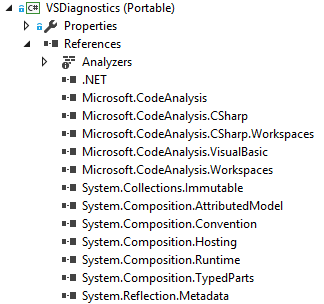
\includegraphics[scale=0.8]{security-analyzers-solution-explorer}
\caption[Analyzers amongst the project dependencies]{Analyzers amongst the project dependencies}
\label{img:security-analyzers-solution-explorer}
\end{figure}

That being said, in the end this is the same risk as with every other piece of software you download. Caution is advised anytime you download something from the internet and it's important to be aware of where things might be hidden.